\section{Additional Figures}

\begin{frame}[label=example_alternative]{Distribution: Example Alternative}
    \begin{figure}
        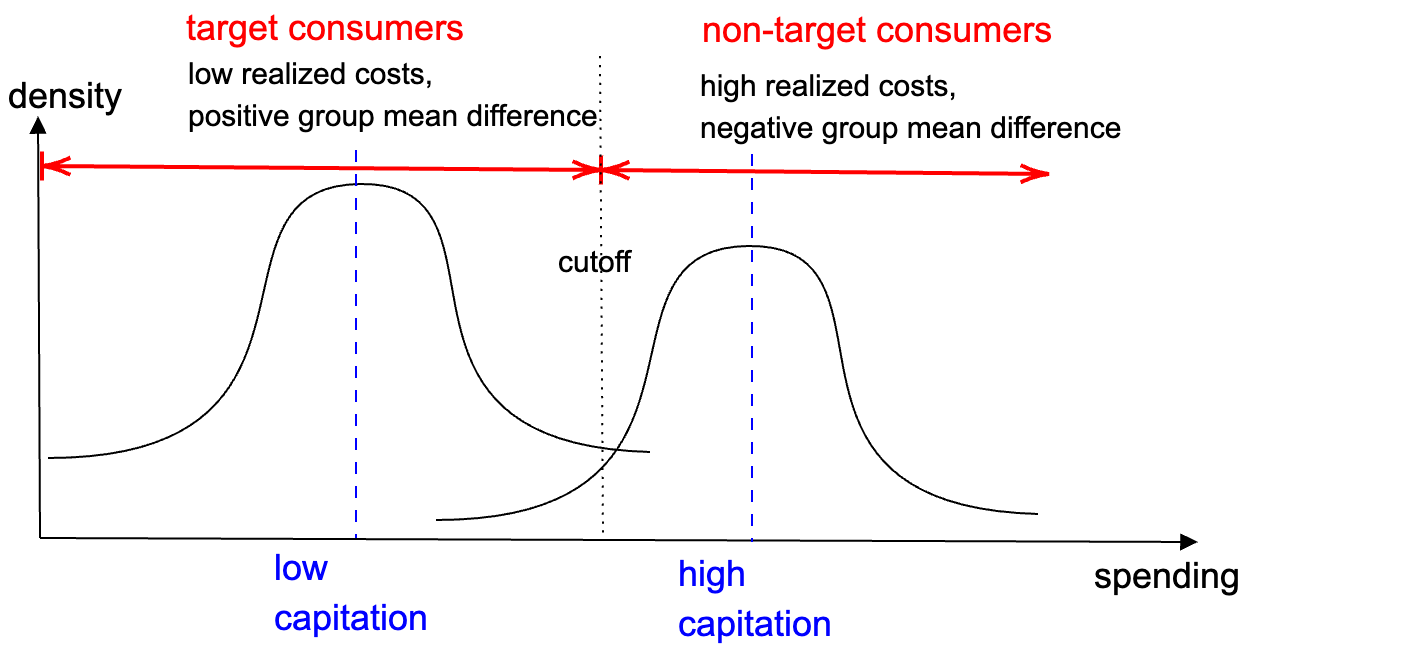
\includegraphics[width=0.8\textwidth]{figures/images/example_2.png}
        \caption{Example Distribution of Capitation and Spending}
    \end{figure}
    \hyperlink{example_distribution}{\beamergotobutton{back Example}}
\end{frame}

\begin{frame}[label=version2]{Sign of Selection: Plan Design}
    \begin{table}[ht]
\centering
\scriptsize
\begin{tabular}{|l|c|c|c|c|}
\hline
\multicolumn{5}{|c|}{\textbf{Medicare Advantage}} \\
\hline
Plan Code & Premium & OOP for Good & OOP for Bad & Additional Benefits \\
\hline
H3370-032 & \$372  & \$1528 & \$10184 & Dental, Vision, Hearing   \\
R5342-001 & \$0 & \$1510 & \$10068 & Vision, Hearing           \\
H4922-001 & \$0 & \$1366 & \$9108 & Dental, Vision           \\
\multicolumn{5}{|c|}{\ldots} \\
\hline
\multicolumn{5}{|c|}{\textbf{Medigap}} \\
\hline
Plan Code & Premium & OOP Good & OOP Bad & Additional Benefits \\
\hline
Plan C & \$3108 & \$0 & \$0 & No\\
\hline
\end{tabular}
\caption{Comparison of MA and Medigap plans in Suffolk County in 2016}
\end{table}

    \hyperlink{version1}{\beamergotobutton{go back}}
\end{frame}

\section{Why Capitation Concentrated}

\begin{frame}[label=example_start]{Conventional Risk Adjustment}
    \begin{itemize}
        \item the risk adjustment currently used
        \item it approximates the average spending for coding combinations
    \end{itemize}
    
\end{frame}

\begin{frame}{Example}
    Coding Combination: e.g. \{\texttt{66, Male, Type II Diabetes}\}
    \begin{figure}
        \centering
        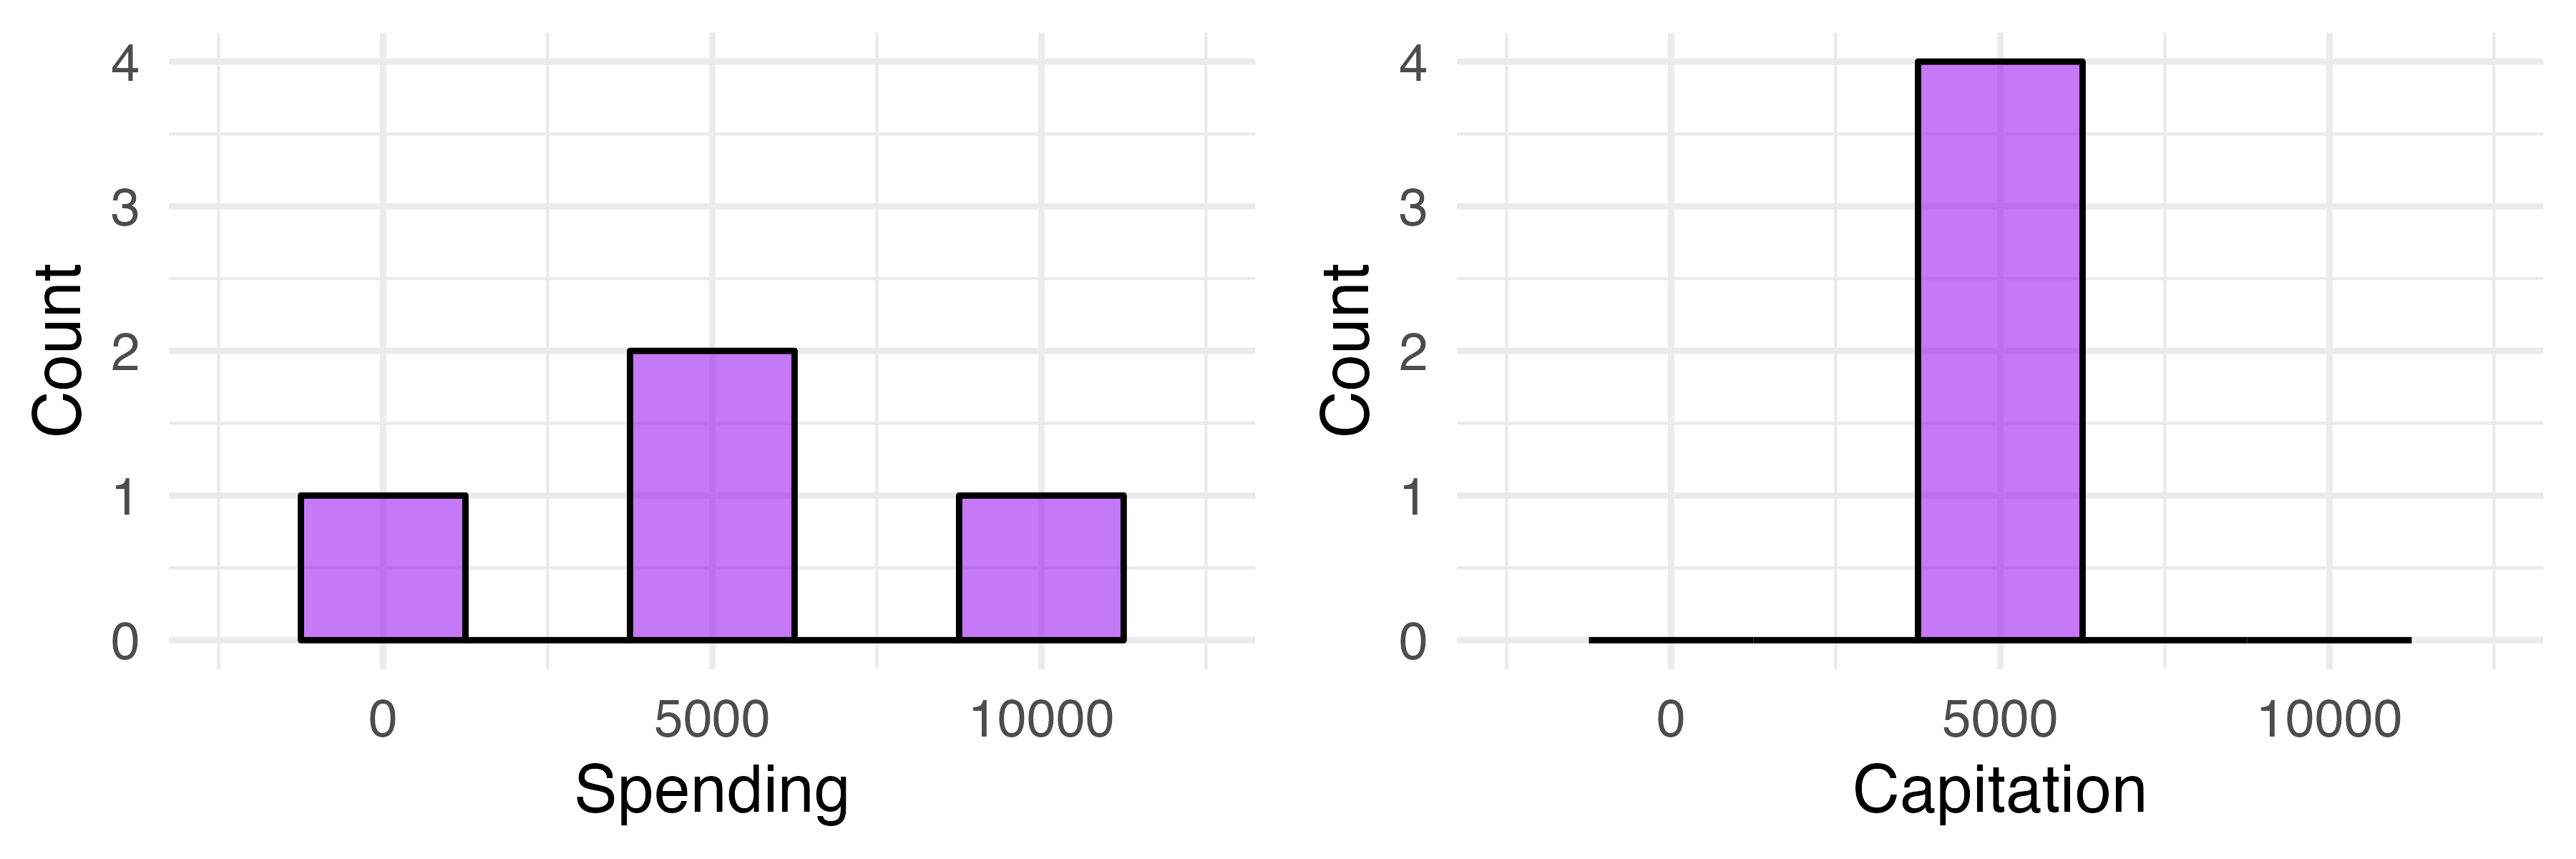
\includegraphics[width=0.8\textwidth]{figures/images/histogram.png}
        \caption{Example Histogram}
    \end{figure}
\end{frame}

\begin{frame}{Implication from Example}
    Conventional Risk Adjustment should have:
    \begin{itemize}
        \item \textbf{Low Dispersion}: more concentrated on the middle
        \item \textbf{Limited Precision}: not a good predictor for individual spending.
    \end{itemize}
\end{frame}
\begin{frame}[label=distribution]{Distribution from Real Data}
    \begin{figure}
        \centering
        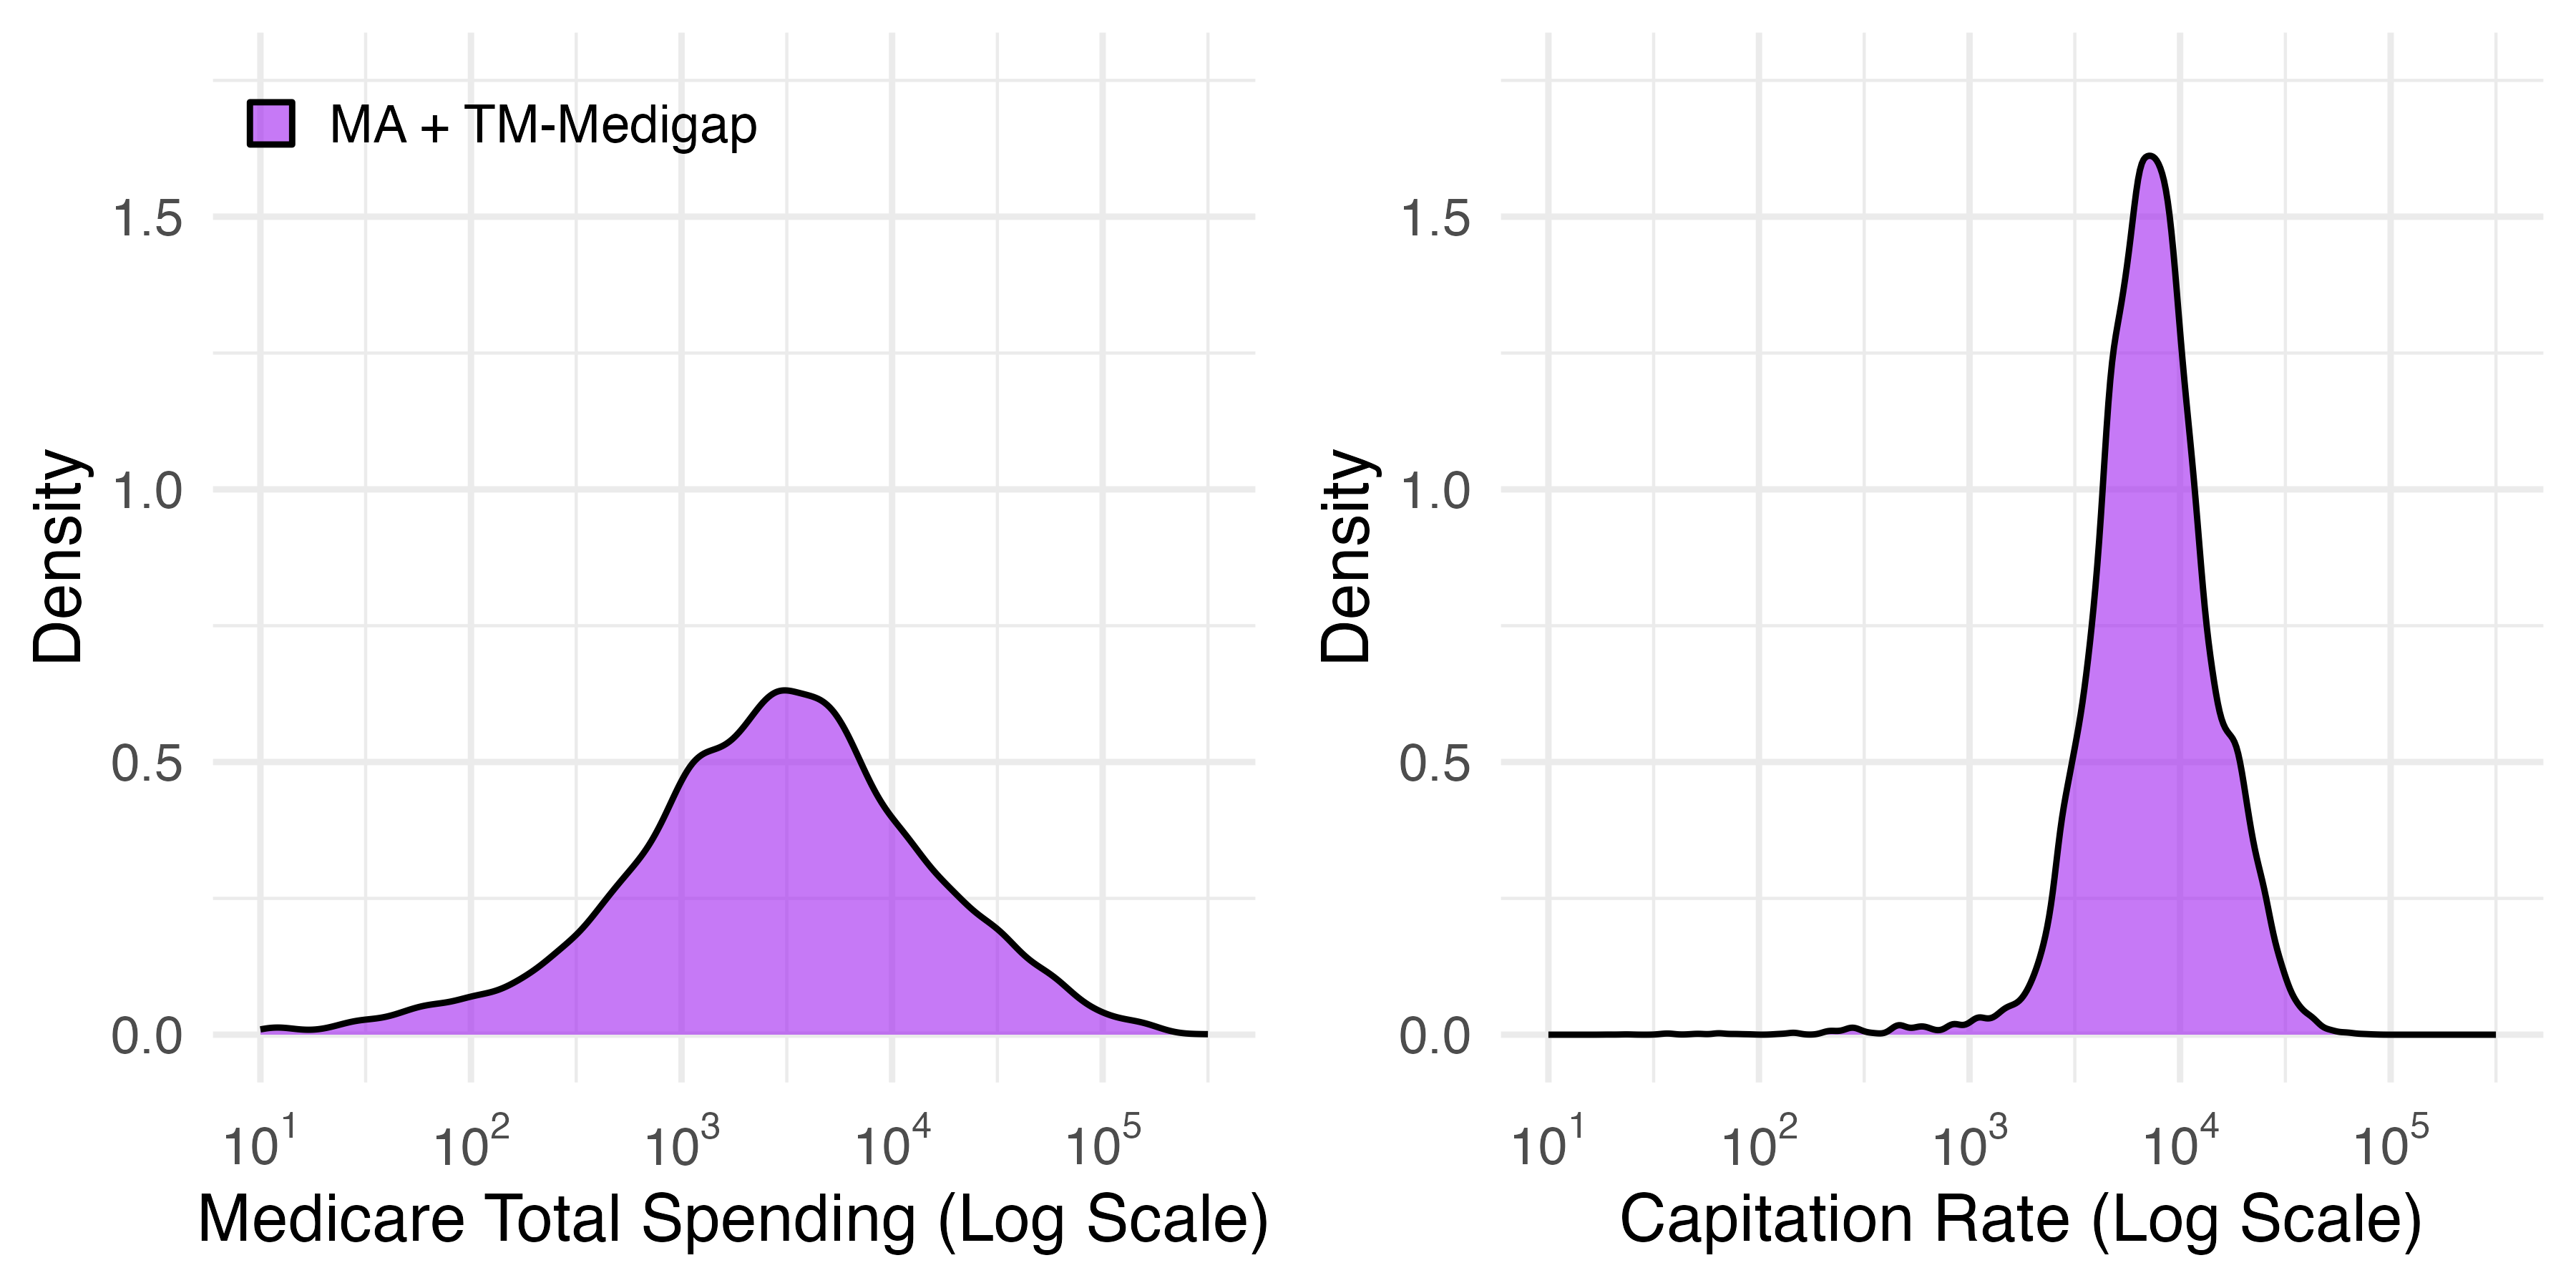
\includegraphics[width=0.8\textwidth]{figures/images/capitation_spending_distribution_ungrouped.png}
        \caption{Distribution of Capitations \& Spending}
    \end{figure}
\end{frame}

\begin{frame}[label=example_end]{Distribution from Real Data}
    Real Data confirms:
    \begin{itemize}
        \item \textbf{Low Dispersion}: more concentrated than payment.
        \item \textbf{Limited Precision}: the offical model's $R^2$ is 0.1 on individual level \footnote{\textit{Report to Congress: Risk Adjustment in MA, 2021}}.
    \end{itemize}
    \vfill
    \hyperlink{source_of_incentive}{\beamergotobutton{back}}
\end{frame}

\section{Overpayment}
\begin{frame}[label=overpayment_distribution]{Result: Overpayment}
    \begin{figure}
        \centering
        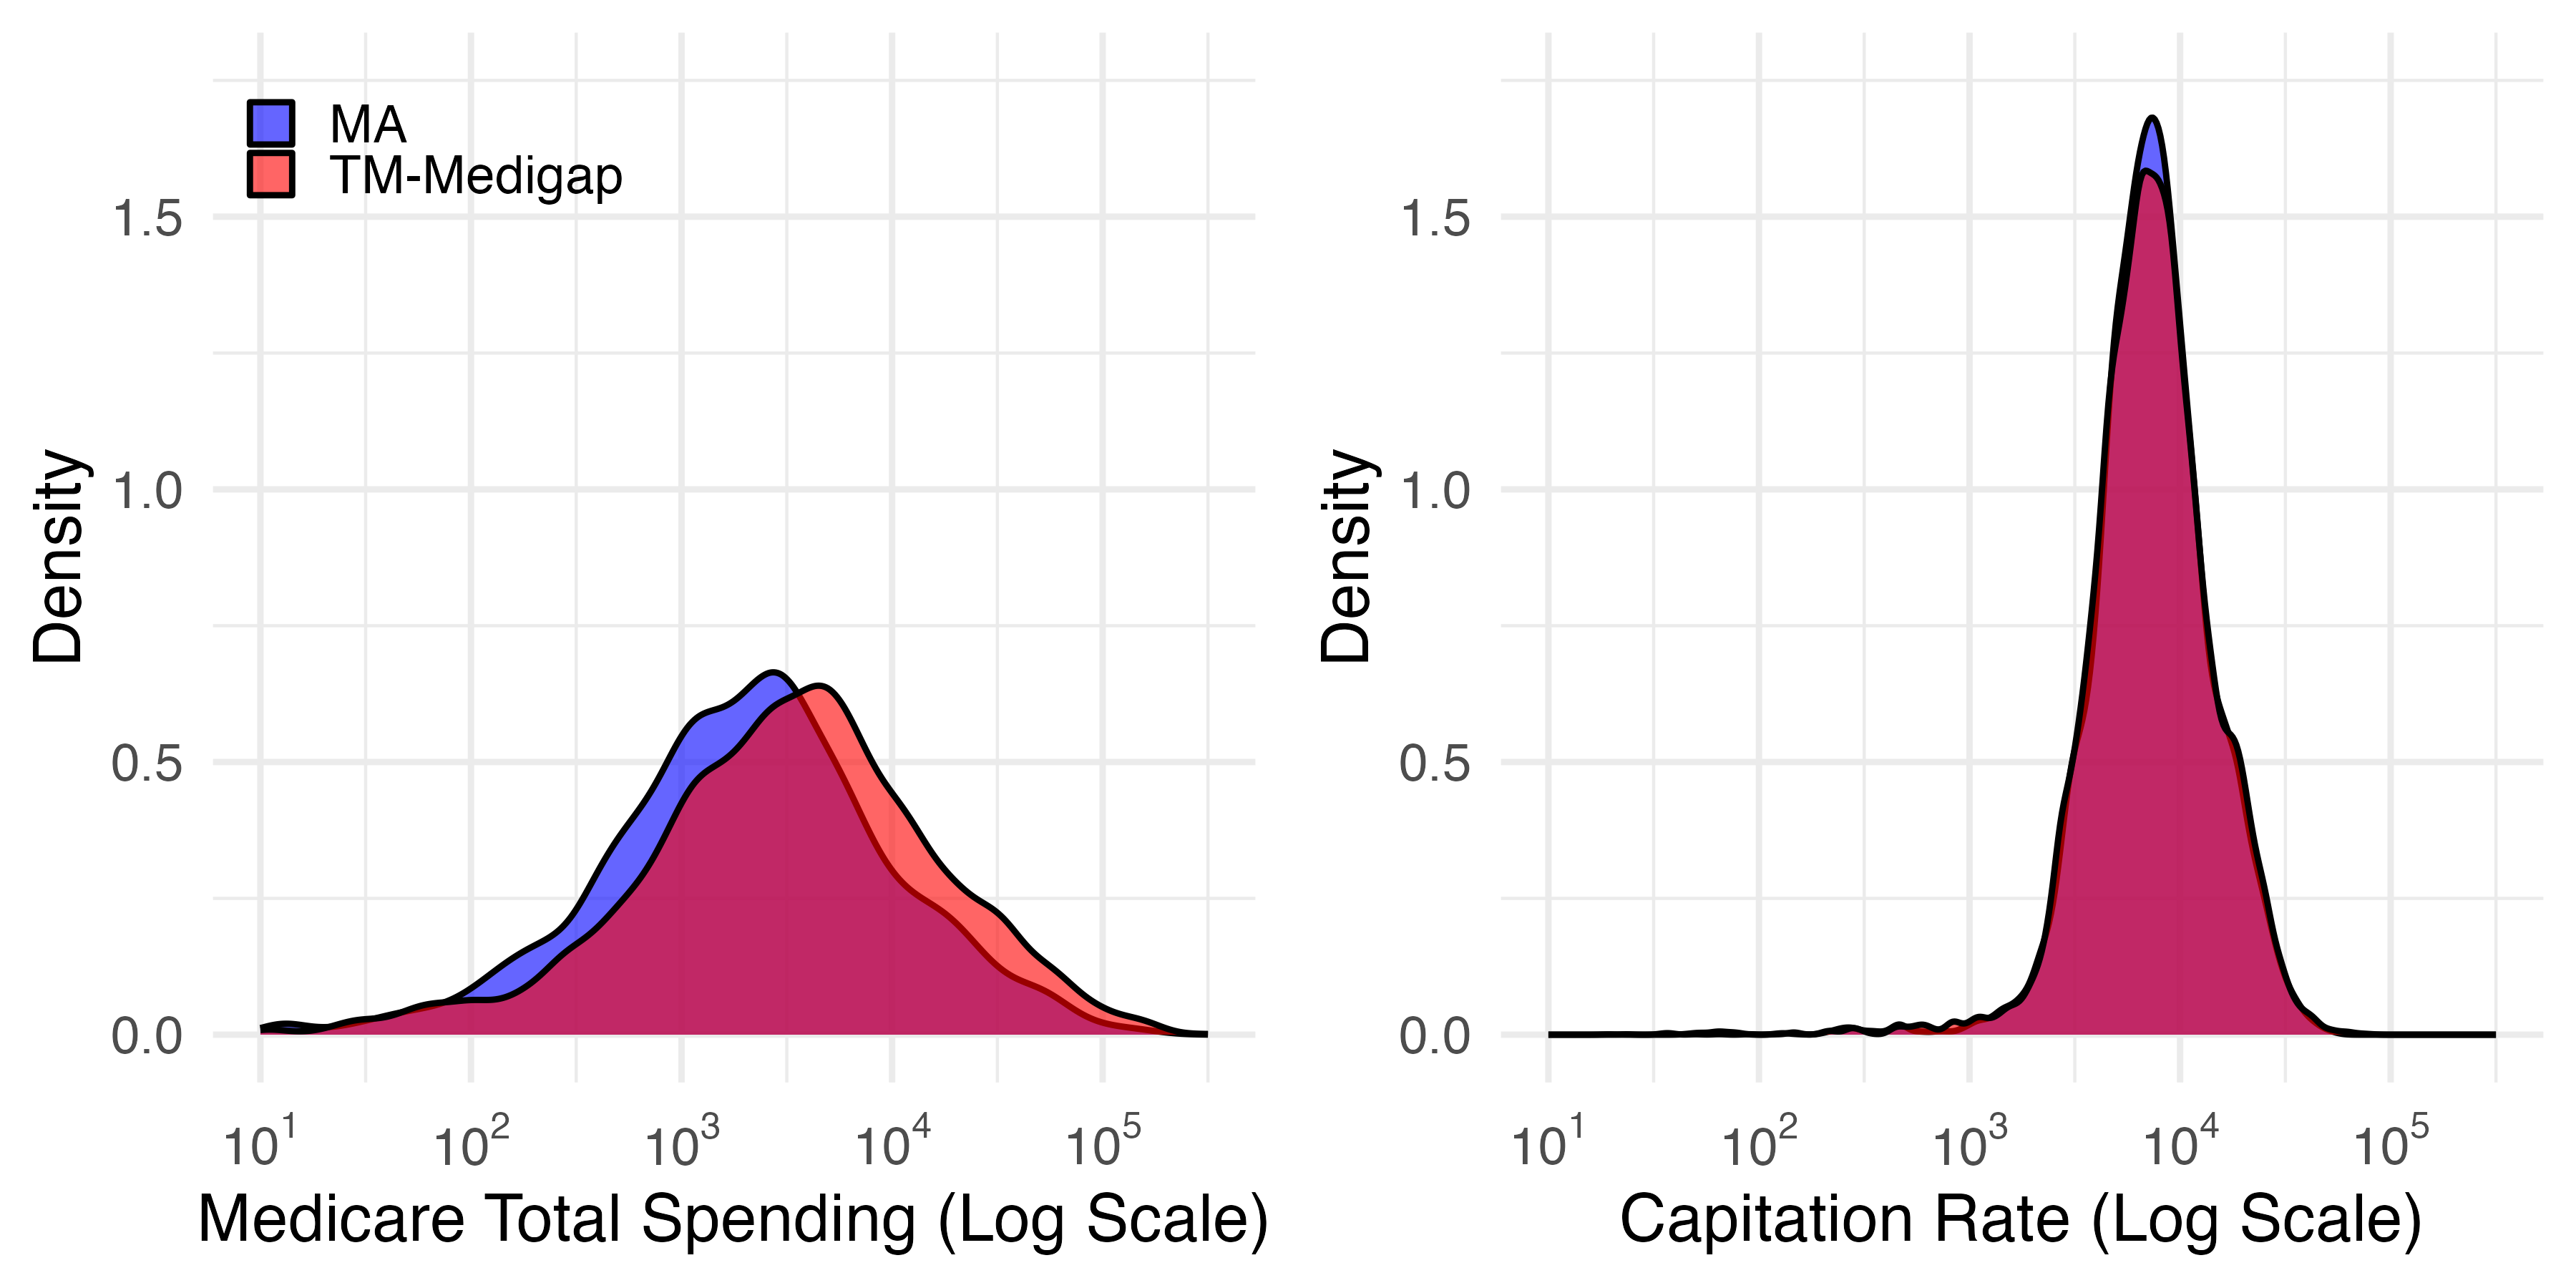
\includegraphics[width=0.8\textwidth]{figures/images/capitation_spending_distribution_grouped.png}
        \caption{Distribution of Capitations \& Payments by Plan Type}
    \end{figure}
    \hyperlink{explain_overpayment}{\beamerbutton{back}}
\end{frame}

\begin{frame}{Result: Overpayment}

    \begin{itemize}
        \item MA and TM have \textit{almost} same distribution of capitation rates.
        \item MA has a higher frequency of low spending, lower of high spending.
        \item This is consistent with our story.
        \item MA firms ``skim cream'' on group level, not individual level.
        \item The root cause is the imperfect risk adjustment.
    \end{itemize}
\end{frame}

\begin{frame}{Individual Level Summary by Plan Type}
    \begin{figure}
        \centering
        \input{figures/tables/personal_level_summary.tex}
    \end{figure}
    \hyperlink{explain_overpayment}{\beamerbutton{back}}
\end{frame}


\subsection*{Zoom Link}
\begin{frame}
    \href{https://stonybrook.zoom.us/j/95094572016?pwd=ejJWMTdNTzVVTFppQjZqM0lzdGFkUT09}{Zoom Link}
\end{frame}